\documentclass[11pt,xcolor=svgnames]{beamer}
\usepackage{amsmath}
\usepackage{amssymb}
\usepackage{amsfonts}
\usepackage{dsfont,natbib,setspace,changepage,multirow}
\usepackage{tikz}
\mode<presentation>

% replaces beamer foot with simple page number
\setbeamertemplate{navigation symbols}{}
\setbeamerfont{frametitle}{series=\bfseries,size=\normalsize}
\setbeamercolor{frametitle}{fg=Black}

\setbeamertemplate{footline}{
  \raisebox{5pt}{\makebox[\paperwidth]{\hfill\makebox[20pt]{\color{gray}\scriptsize\insertframenumber}}}}

\usepackage{algorithm}
\usepackage{algorithmic}

% colors
\newcommand{\theme}{\color{DarkRed}}
\newcommand{\bk}{\color{black}}
\newcommand{\rd}{\color{red}}
\newcommand{\fg}{\color{ForestGreen}}
\newcommand{\bl}{\color{blue}}
\newcommand{\gr}{\color{black!50}}
\newcommand{\sg}{\color{DarkSlateGray}}
\newcommand{\nv}{\color{Navy}}
\setbeamercolor{itemize item}{fg=gray}

% common math markups
\newcommand{\bs}[1]{\boldsymbol{#1}}
\newcommand{\mc}[1]{\mathcal{#1}}
\newcommand{\mr}[1]{\mathrm{#1}}
\newcommand{\bm}[1]{\mathbf{#1}}
\newcommand{\ds}[1]{\mathds{#1}}
\newcommand{\indep}{\perp\!\!\!\perp}
\def\plus{\texttt{+}}
\def\minus{\texttt{-}}
\DeclareMathOperator*{\argmin}{arg\,min}

% spacing and style shorthand
\setstretch{1.1}

\title{Persado Email Subject Lines Project}
\subtitle{Digital and Algorithmic Marketing (37304-01)}
\author{Brian Chingono, Will Clark, Matthew DeLio, Jonathan Stevens}
\institute{
\includegraphics[width=0.5\textwidth]{university_of_chicago_booth_business_school.png}}
\date{\today}

\begin{document}

\begingroup % remove page number from title slide (probably a simpler way to get this done but it works)
\renewcommand{\insertframenumber}{}
 \begin{frame}
  \addtocounter{framenumber}{-1}
  \titlepage
 \end{frame}
\endgroup

% Didn't want on title page because we'd duplicate the phoenix
\usebackgroundtemplate{%
\tikz\node[opacity=0.9] {
	
\includegraphics[height=\paperheight]{phoenix}};
}
% \usebackgroundtemplate{
\includegraphics[height=\paperheight]{phoenix}}


\begin{frame}

Modeling objectives:
\begin{itemize}
\item Predict click behavior out of sample\\\textit{\fg select variables via cross validation}
\item Prefer simplicity/parsimony to complexity\\\textit{\fg choose a small model}
\item Main effects matter more than interaction effects\\\textit{\fg impose a bias toward main effects}
\end{itemize}

\end{frame}

\begin{frame}

The model:
\[ \log\left[\frac{\textsf{Pr}(\text{click}=1)}{1-\textsf{Pr}(\text{click}=1)}\right] = \beta_0 + \underbrace{\sum_{j=1}^{p} x_j \beta_j}_{\text{main effects}} + \underbrace{\sum_{j=1}^p \sum_{k=1}^{j-1} x_j x_k \beta_{jk}}_{\text{interaction effects}} + \varepsilon \]

The lasso:
\[ \min_{\bm{\beta}} \left(-\frac{2}{n}\log{\textsf{LHD}(\bm{\beta})} + \underbrace{\lambda \sum_{i} \vert \beta_i \vert}_{\text{main + int. effects}} \right) \]
% Note: strictly speaking the first term is *proportional* to the deviance and the second term is *proportional* to the absolute value

\vskip 0.25cm \nv 
We can vary the weight on $\lambda$ to impose different shrinkage for different variables!

\end{frame}

\begin{frame}

The lasso with a twist:
\[ \min_{\bm{\beta}} \left(-\frac{2}{n}\log{\textsf{LHD}(\bm{\beta})} + \underbrace{\omega_1 \lambda \sum_{j=1}^{p} \vert \beta_j \vert}_{\text{main effects}} + \underbrace{\omega_2 \lambda \sum_{j=1}^p \sum_{k=1}^{j-1} \vert \beta_{jk} \vert}_{\text{interaction effects}} \right) \]

\vskip 0.5cm 
$\omega_1 < \omega_2$: the lasso will penalize interaction effect parameters more than main effect parameters (\textit{\fg impose a bias toward main effects})

\end{frame}

% \begin{frame}
% Trade-off between accuracy (\textit{\fg select variables via cross validation})...
% 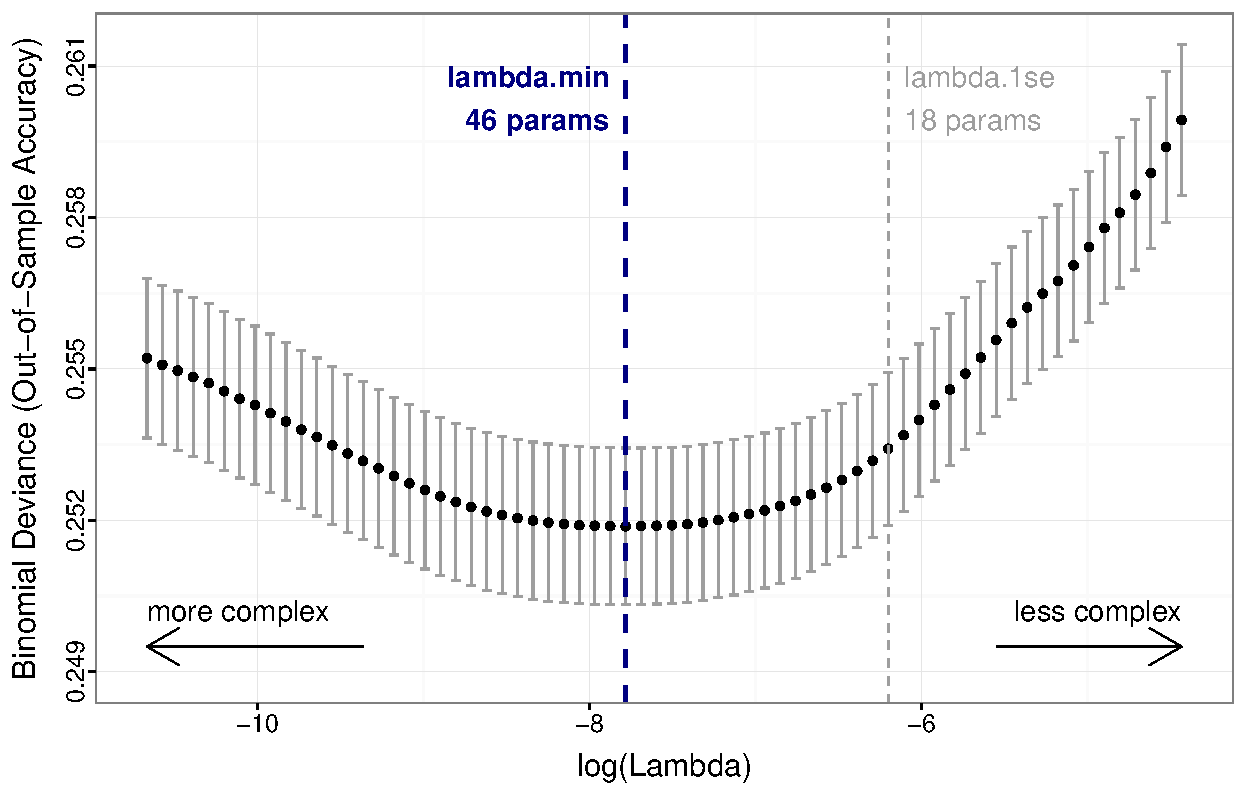
\includegraphics[width=\textwidth]{regpath1.pdf}
% \end{frame}

\begin{frame}
Trade-off between accuracy (\textit{\fg select variables via cross validation}) and simplicity/parsimony (\textit{\fg choose a small model})
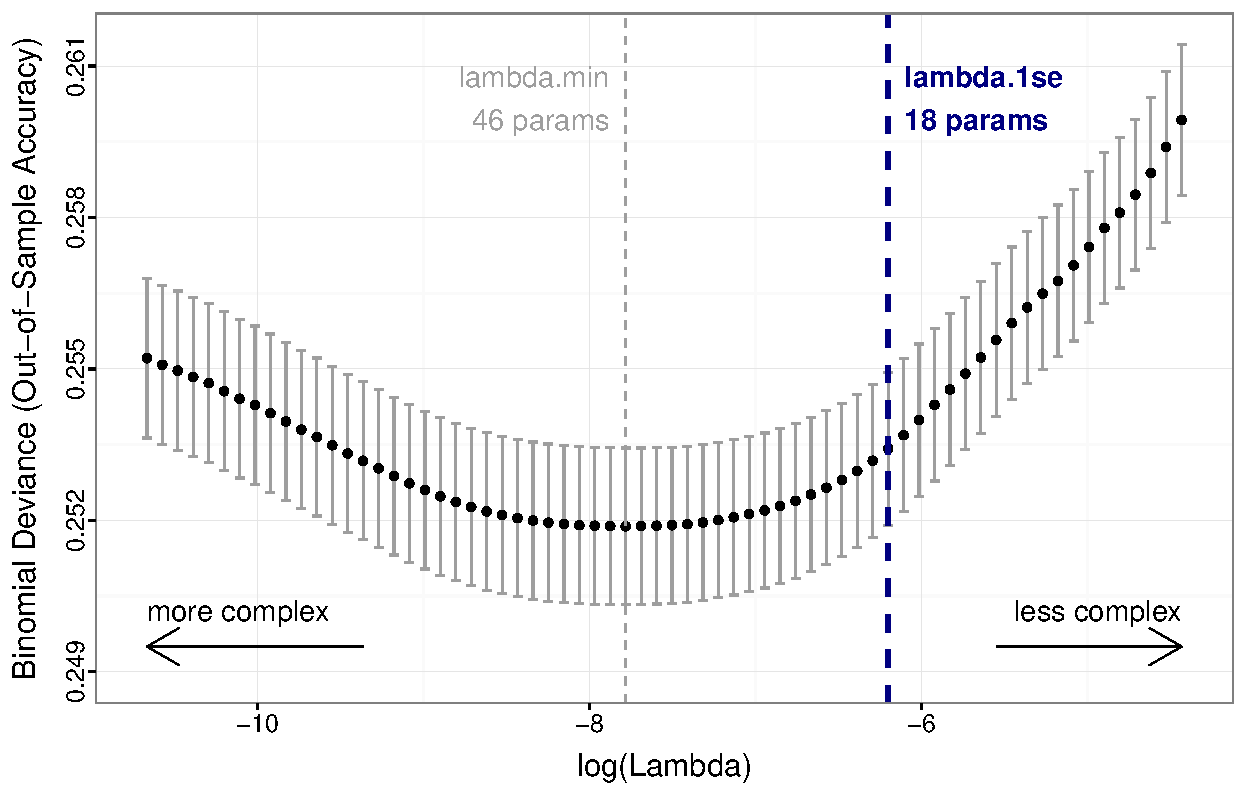
\includegraphics[width=\textwidth]{regpath2.pdf}
\end{frame}

\begin{frame}
The LASSO selects the following coefficients which align with our modeling goals ({\fg small model} \& {\fg main effects})
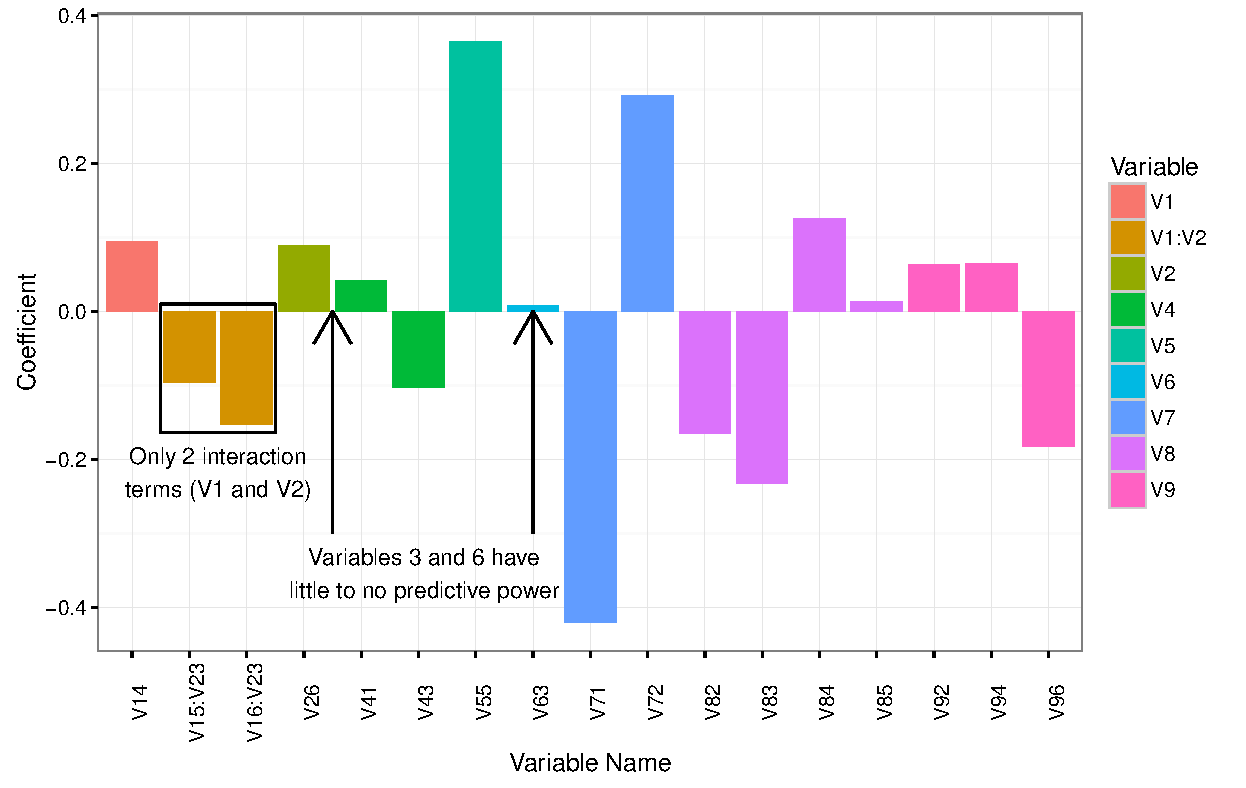
\includegraphics[width=\textwidth]{coef_all.pdf}
\end{frame}

\begin{frame}
We can then estimate this model on our sample of 5 million customers to build predictive capability
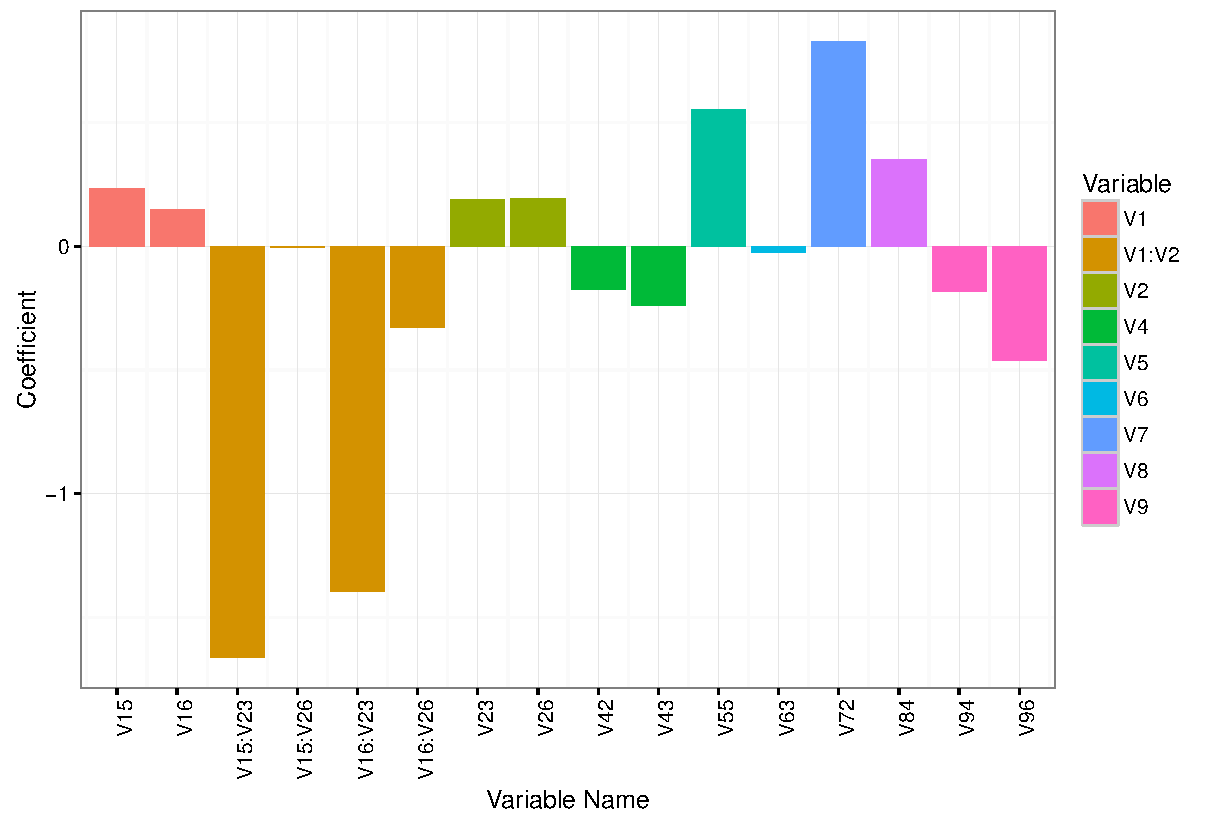
\includegraphics[width=\textwidth]{final_model_coefs.pdf}
\end{frame}

\begin{frame}
The estimated model can find the messages with the best predicted click rate (even among those we have not tested)
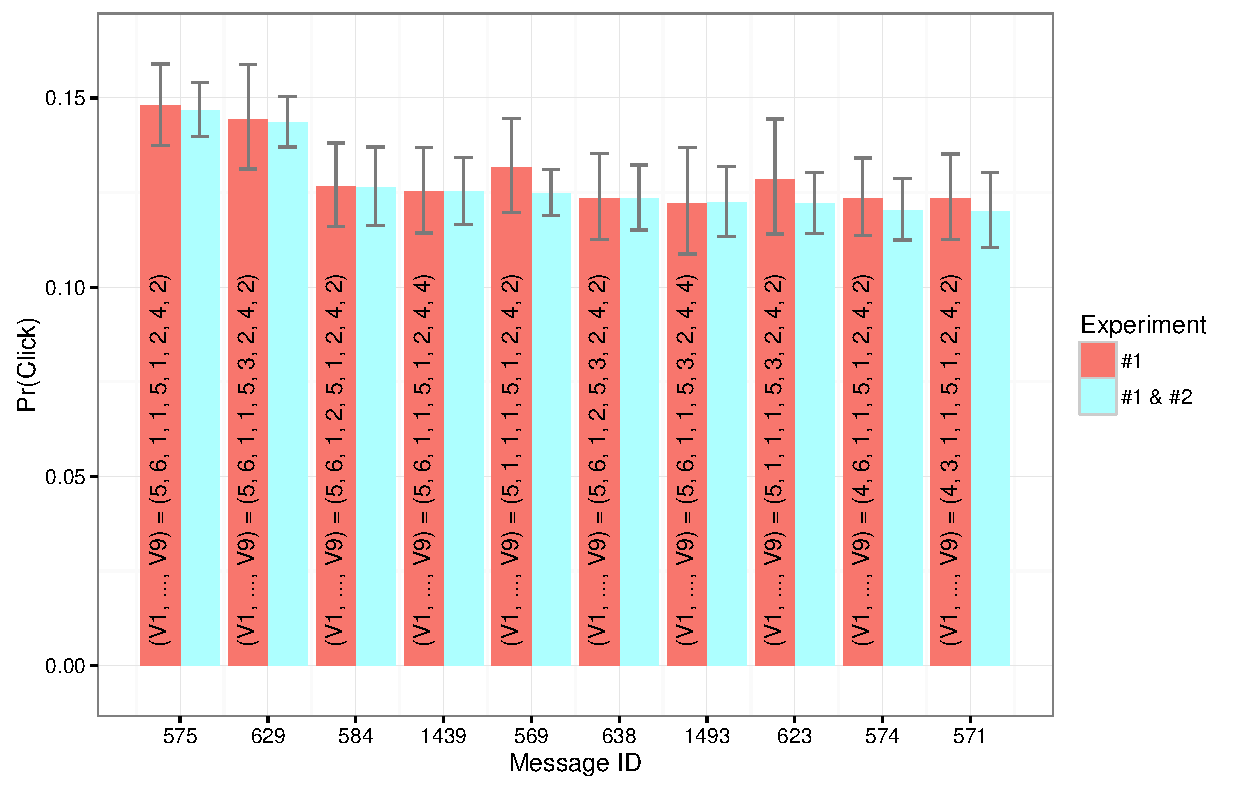
\includegraphics[width=\textwidth]{barplot1.pdf}
\end{frame}

\begin{frame}
To validate model performance (and maybe learn more about V6), we can run a small experiment with two of the top messages
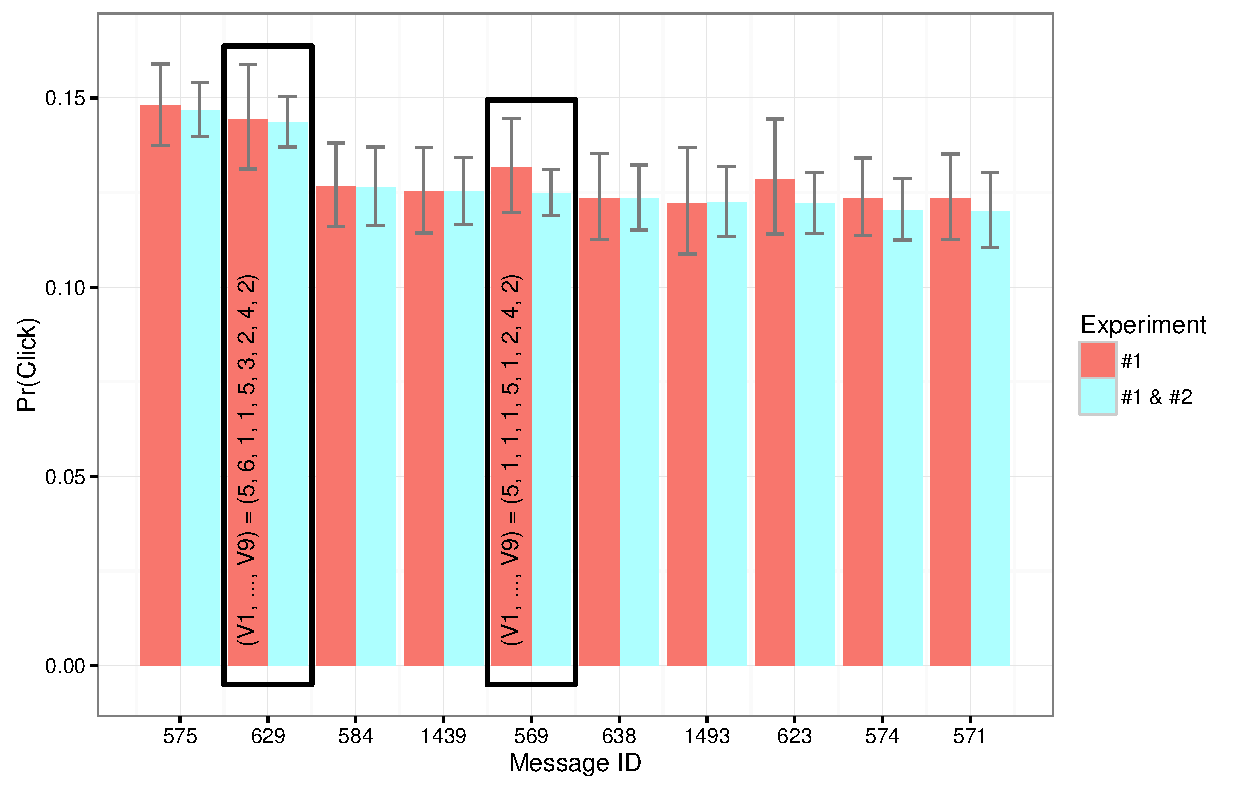
\includegraphics[width=\textwidth]{barplot2.pdf}
\end{frame}

\begin{frame}
With the results of the second experiment, we can re-estimate our model and update our predictions
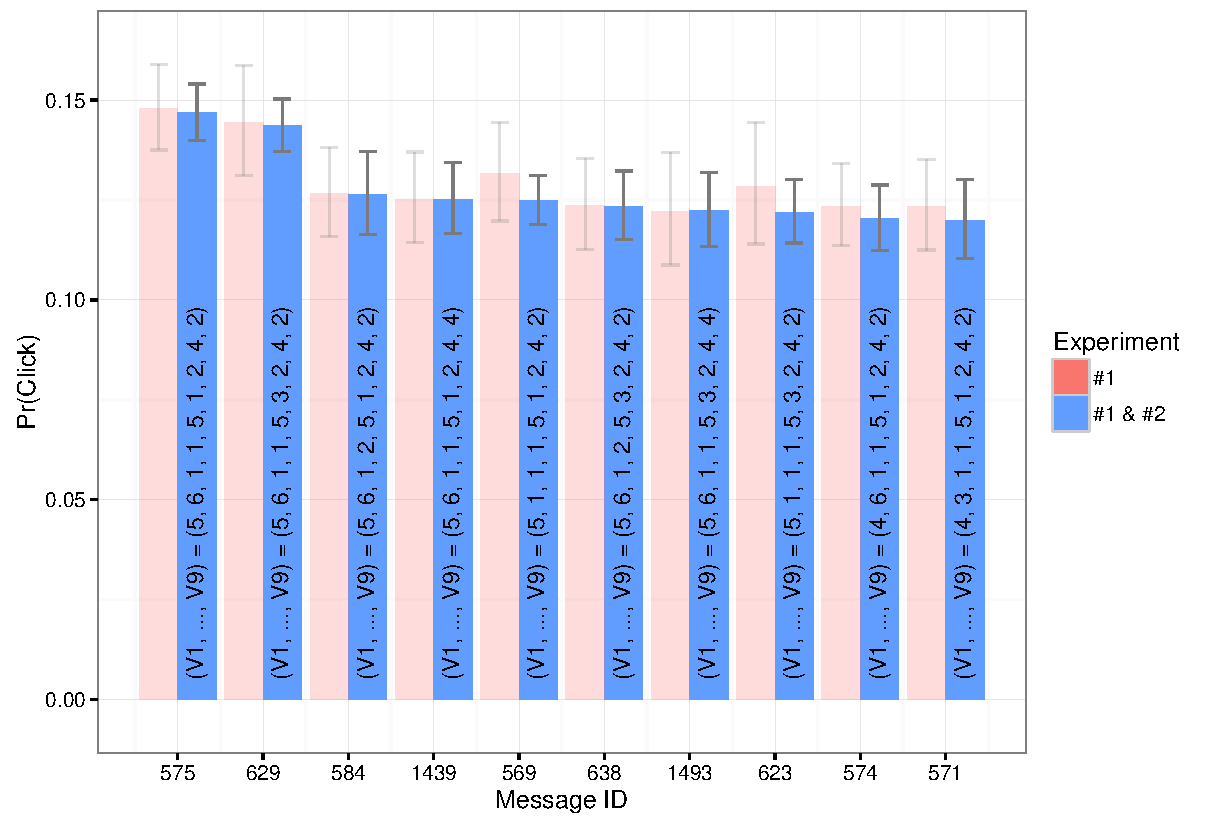
\includegraphics[width=\textwidth]{barplot3.pdf}
\end{frame}

\begin{frame}
Our re-estimated model suggests Message 575 will have the highest click rate (but not by much!)
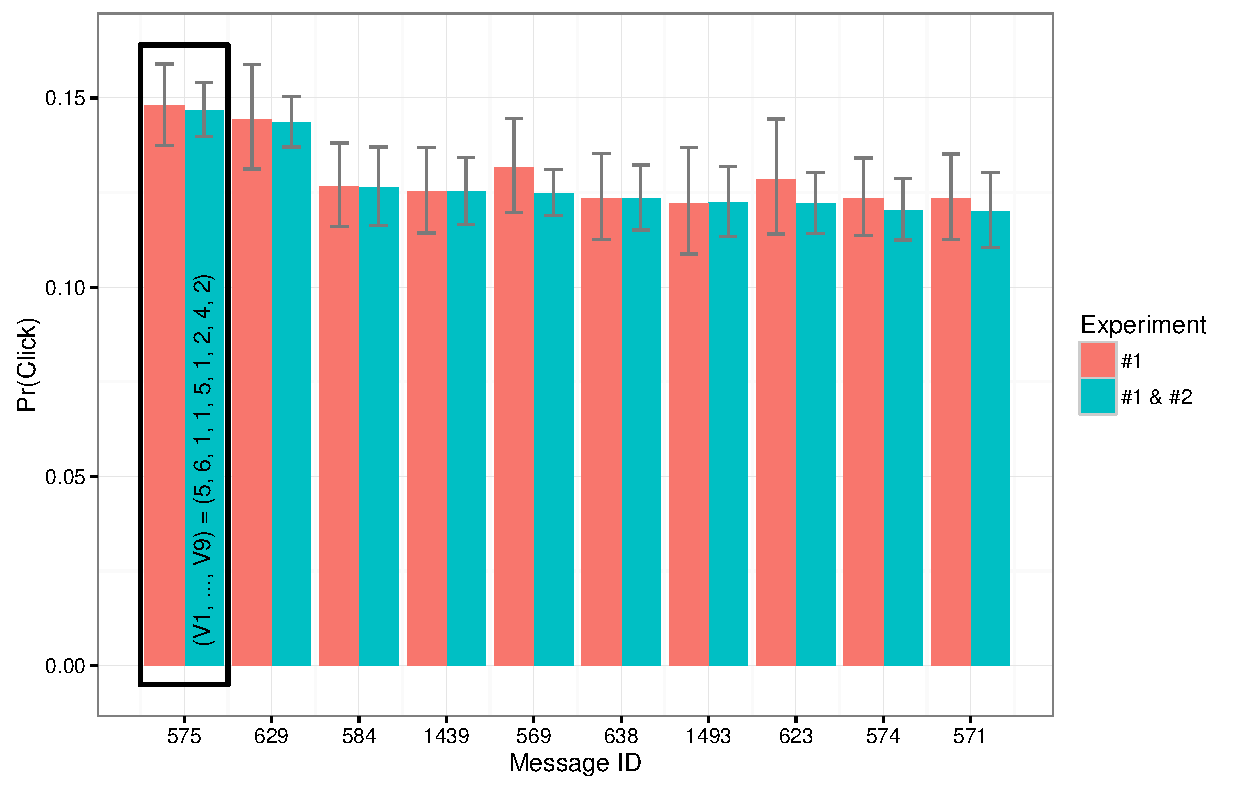
\includegraphics[width=\textwidth]{barplot4.pdf}
\end{frame}


\begin{frame}
\textbf{\Large \nv In conclusion}\\
\vspace{0.2in}
Final message\\
(V1, ..., V9) = (5, 6, 1, 1, 5, 1, 2, 4, 2)\\
\vspace{0.15in}
Predicted click rate: 14.68052 percent\\
{\fg Predicted profit: \$65,886.13}\\
\vspace{0.15in}
95 percent confidence interval\\
(13.98531, 15.40410)\\
{\fg (\$62,573.74, \$69,333.70)}
\end{frame}

\begin{frame}[c]{ }
\centering
Appendix
\end{frame}

\begin{frame}
We observe all variables about in about 75-80 percent of historical experiments
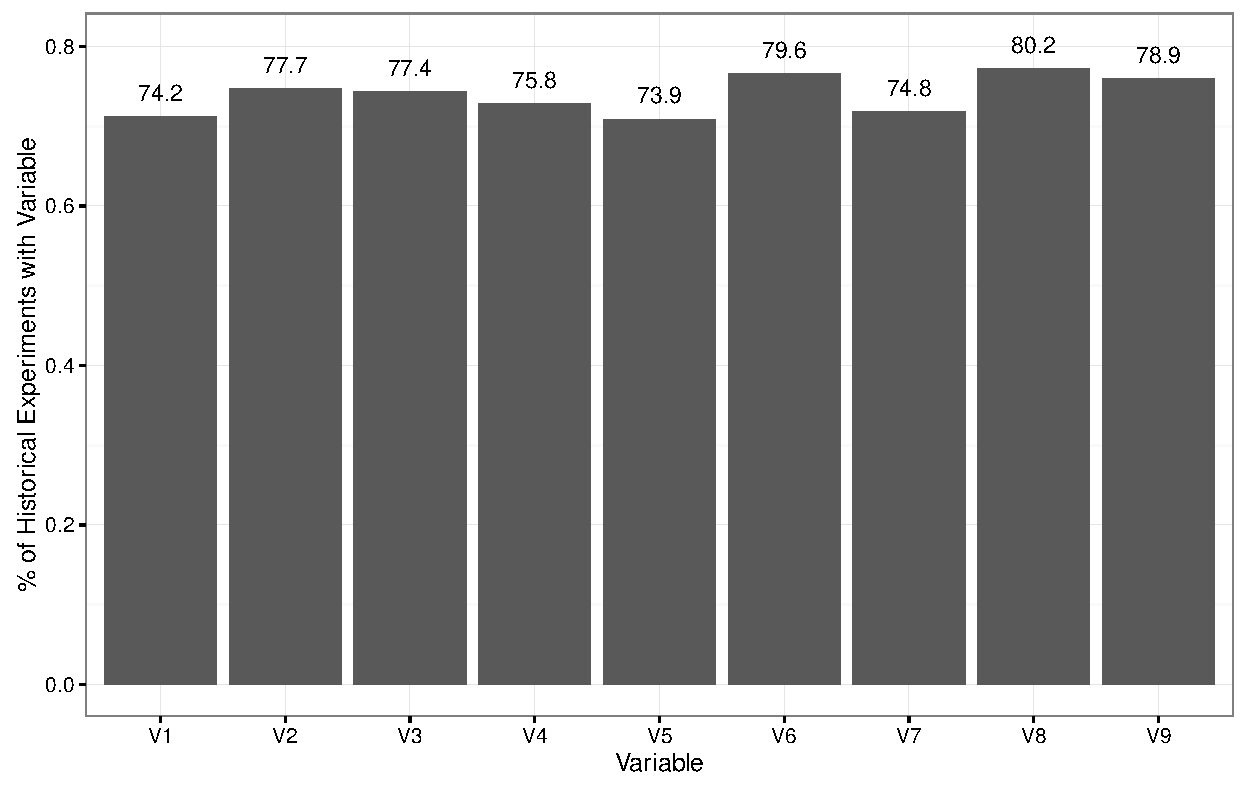
\includegraphics[width=\textwidth]{hist_freq.pdf}
\end{frame}

\begin{frame}
How much better does our model get after the second experiment?
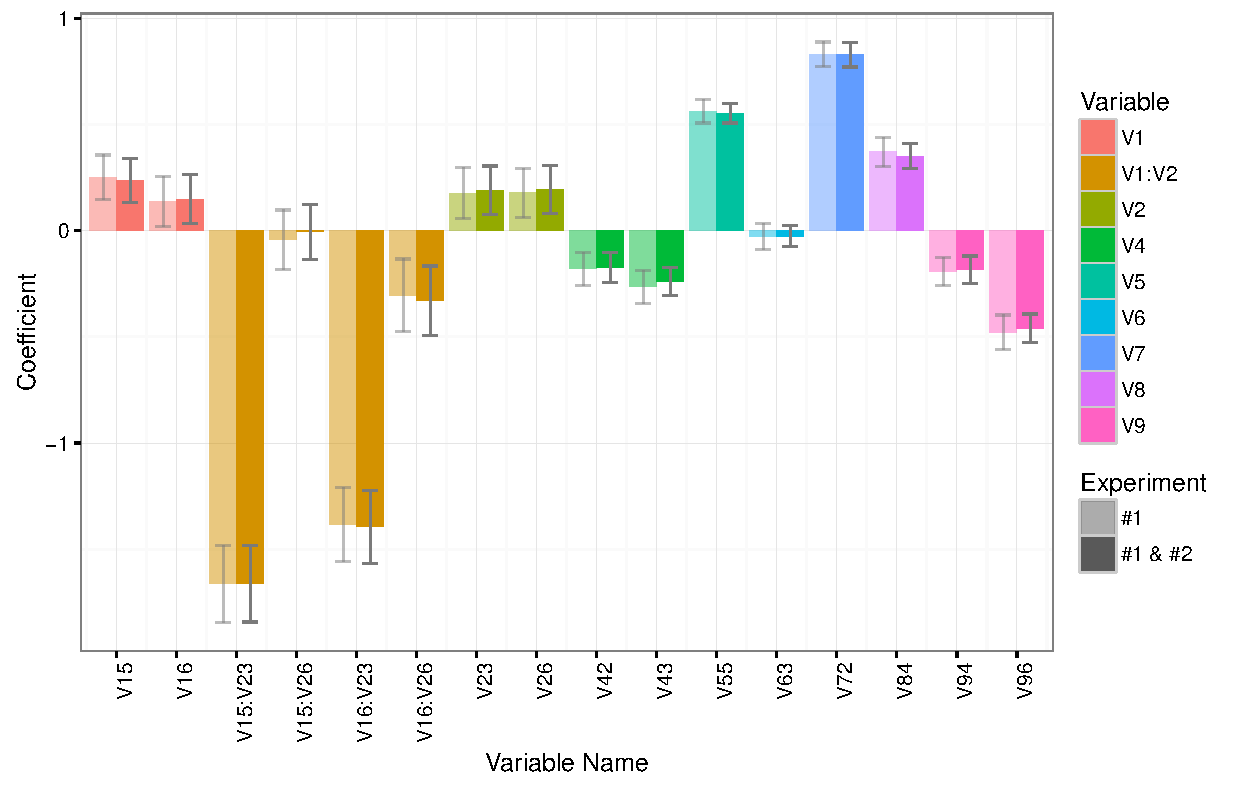
\includegraphics[width=\textwidth]{final_model_coefs_crazy.pdf}
\end{frame}

\begin{frame}
Experimental Model Coverage
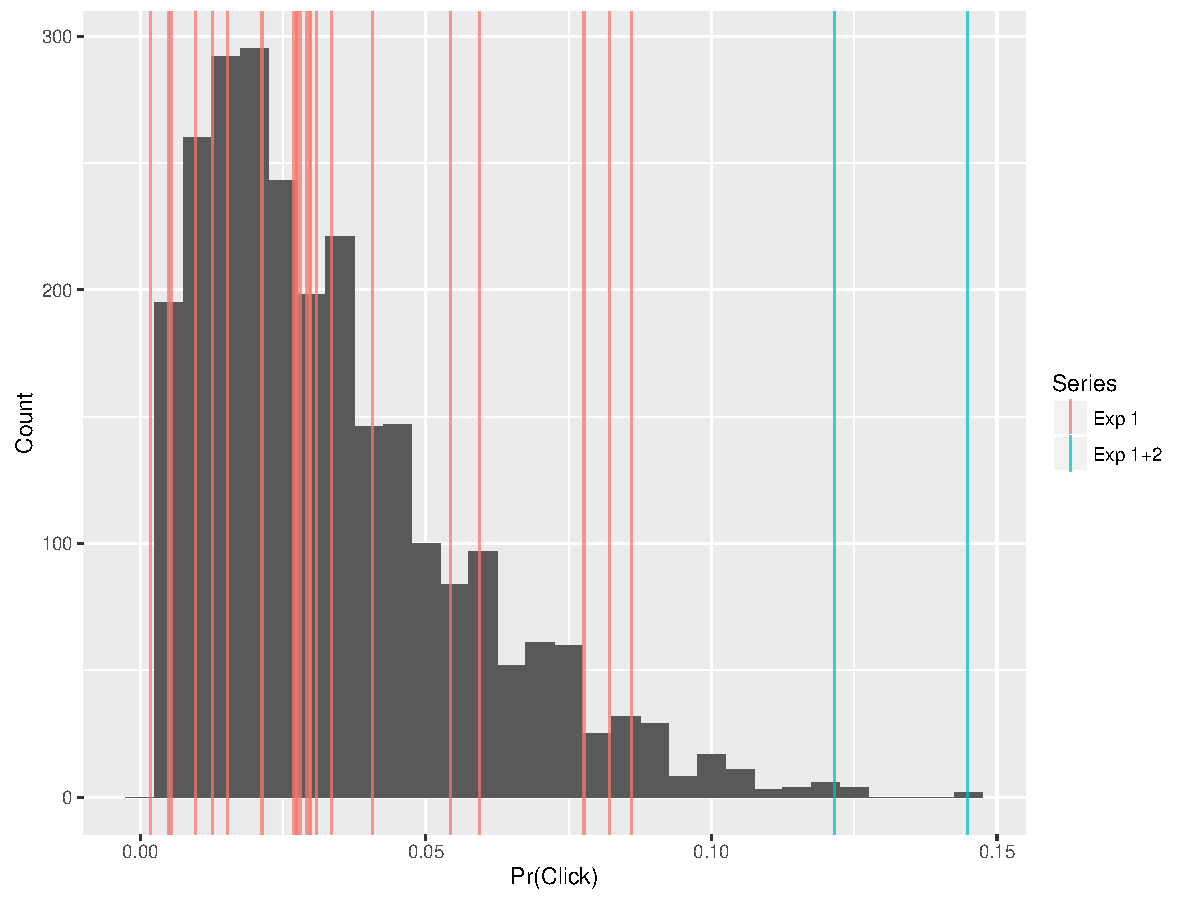
\includegraphics[width=\textwidth]{hist.pdf}
\end{frame}

\end{document}
